% !TeX program = xelatex
% Complete English manuscript. CAS template defaults + native review spacing.
\providecommand{\PaperRoot}{./}
\makeatletter\edef\input@path{{\PaperRoot}{\PaperRoot template/}}\makeatother
\documentclass[a4paper,fleqn,review]{cas-sc}
\usepackage[numbers,sort&compress]{natbib}
\usepackage{bm,tabularx,algorithm,algpseudocode,placeins}
\graphicspath{{\PaperRoot}}
\newcommand{\R}{\mathbb R}
\newcommand{\C}{\mathbb C}
\newcommand{\E}{\mathbb E}
\newcommand{\Rea}{\operatorname{Re}}
\newcommand{\tr}{\operatorname{tr}}
\begin{document}
\let\WriteBookmarks\relax
\shorttitle{Efficient direct localization of overlapping wideband sources}
\shortauthors{}
\title[mode=title]{Efficient direct localization of overlapping wideband sources with unequal powers: multi-candidate joint refinement and waveform-eliminated updates}
% Author names, affiliations, corresponding author, funding and declarations
% must be supplied and confirmed by the authors before submission.
\begin{abstract}
Localizing unknown wideband emitters from mixed observations becomes difficult when their spectra overlap and their received powers differ. Direct position determination fits the station observations jointly, but its reliability and cost depend on candidate selection and position refinement. This paper studies two improvements for synchronized single-antenna stations under a known relative-amplitude and baseband-delay model. Multi-candidate joint-refinement alternating projection (MCJ-AP) retains several conditional candidates, jointly refines both positions for each branch, and selects the smallest final residual. Waveform-eliminated block Newtonized orthogonal matching pursuit (VP-BNOMP) re-estimates the current source coefficients at each trial position and uses the resulting reduced curvature. Across 2,400 observations from 20 source configurations, five-candidate MCJ-AP increases the two-source success rate within 20 m from 95\% to 99\%, with the recoveries concentrated in one configuration. At matched candidates and stopping accuracy, joint refinement reduces mean complete runtime by 31.36\%. In 240 paired observations, reduced curvature lowers mean runtime by 83.77\% relative to fixed-coefficient curvature with the same waveform-eliminated acceptance objective. On 480 observations from 16 new source configurations, both single- and five-candidate AP succeed throughout, whereas VP-BNOMP succeeds in 81.25\%. The results identify the conditional reliability benefit of candidate retention and the computational benefit of removing position--waveform coupling from local updates.
\end{abstract}
\begin{keywords}
Direct position determination\sep Overlapping sources\sep Alternating projection\sep Block NOMP\sep Variable projection
\end{keywords}
\maketitle

\FloatBarrier
\section{Introduction}
Emitter localization often estimates time differences of arrival before solving for position. Generalized correlation and hyperbolic localization provide established tools for this two-step approach \cite{KnappCarter1976,ChanHo1994}. When unknown emitters occupy the same frequency band, each station receives a mixture with different propagation responses. Extracting and associating individual delays then becomes difficult, particularly for a weak emitter in the presence of a stronger one. Direct position determination (DPD) incorporates propagation into the observation model and estimates positions from the station data jointly \cite{ChenHudsonYao2002,WeissAmar2005}.

This paper considers two independent unknown wideband sources observed by four synchronized single-antenna stations. The positions, transmitted waveforms and powers are unknown; station coordinates and relative propagation responses are available. A single-source spectrum can assign several large peaks to the stronger source, whereas an exhaustive search over two two-dimensional positions requires many combinations. Sequential discovery followed by continuous refinement reduces this search, but leaves two decisions: which candidate regions to retain, and how to update positions while estimating the unknown waveforms.

Wideband maximum likelihood and alternating projection (AP) reduce joint search dimensionality by updating one position conditional on the others \cite{ChenHudsonYao2002}. MUSIC-type DPD uses orthogonality to an estimated noise subspace \cite{WeissAmar2005}. MVDR uses the inverse covariance to suppress interfering components \cite{Capon1969}, and DPD-HR applies this principle to direct localization \cite{TirerWeiss2016}. These methods process mixtures differently, and their relative performance also depends on covariance estimation and search. We therefore compare concrete implementations using the same data and propagation information.

Newtonized orthogonal matching pursuit (NOMP) combines greedy discovery, Newton refinement and cyclic updates \cite{Mamandipoor2016}. The two-dimensional multi-frequency block NOMP of Yang et al. groups the unknown frequency coefficients at a common position and re-estimates them after position updates \cite{Yang2022}. It supplies a close reference for the local update studied here. QNOMP eliminates path gains and jointly refines delays and angles from pilot-based channel observations \cite{Zeng2025}. In our model the unknown coefficients are the per-frequency amplitudes of independent source waveforms, and the nonlinear parameters are source positions.

Candidate selection also has relevant precedents. Oh and Un use sequential MUSIC initialization before AP updates \cite{OhUn1991}. LAOLS retains discrete atom candidates and completes a tentative support before comparing its residual \cite{Chatterjee2012}. Here, a conditional spectrum holds the first position fixed, while continuous joint refinement allows both positions to move. The two operations can rank branches differently. Retaining several conditional candidates delays the decision until after continuous fitting, without repeating the full spatial scan for each branch.

The treatment of unknown waveforms affects refinement cost as well. Variable projection eliminates linear coefficients before optimizing nonlinear parameters \cite{GolubPereyra1973}. We apply this principle to local block-NOMP position updates and examine the curvature term removed by waveform re-estimation. The paper makes two methodological contributions:
\begin{enumerate}
\item MCJ-AP compares conditional candidates after joint continuous refinement. Candidate retention improves initialization coverage, while joint updates reduce the cost of processing the retained branches at a common stopping accuracy.
\item VP-BNOMP retains residual discovery and cyclic block updates, but eliminates the current source waveform during each local position trial. A curvature analysis and a paired comparison with the same acceptance objective isolate its effect on repeated small updates.
\end{enumerate}
Experiments compare eight method families on a common 240-observation subset, examine the principal methods on 2,400 observations, and test frozen configurations on 480 observations at new source positions. The receiver coordinates remain fixed. These experiments distinguish candidate recovery from local computational savings.

\FloatBarrier
\section{Observation model and localization objective}
\FloatBarrier
\subsection{Synchronized wideband observations}
Let $\bm r_l\in\R^2$ denote station $l$, $l=1,\ldots,L$, and let $\bm p_k\in\Omega\subset\R^2$ denote source $k$, $k=1,\ldots,K$. We assume static direct-path propagation, synchronized station timing and frequency, calibrated relative receiver responses, and matched antenna polarization with equal directional responses. The experiments use $L=4$ and known $K=2$. Define
\begin{equation}
d_{lk}=\|\bm p_k-\bm r_l\|_2,\qquad
\tau_{lk}=d_{lk}/c_0,\qquad \beta_{lk}=d_{lk}^{-1},
\label{en:distance}
\end{equation}
where $c_0$ is propagation speed. For far-field, matched isotropic antennas, free-space attenuation gives
\begin{equation}
P_{\rm r}/P_{\rm t}=(\lambda/4\pi d)^2,\qquad
a_{\rm amp}(d)=\sqrt{P_{\rm r}/P_{\rm t}}=\lambda/(4\pi d).
\label{en:freespace}
\end{equation}
Here $P_{\rm r}$ and $P_{\rm t}$ are received and transmitted powers, and $\lambda$ is wavelength \cite{ITURP5252024}. With fixed $\lambda$ and antenna responses, the common factor $\lambda/(4\pi)$ is absorbed into the unknown waveform, leaving relative amplitudes proportional to $1/d$.

The propagation phase is specified by an ideal baseband pure-delay model. Receiver calibration removes station responses; it does not establish this propagation assumption. Both generator and estimators use the same baseband model, without an RF carrier phase or random link gains. With sampling rate $f_s$ and $N$ samples,
\begin{equation}
x_l[n]=\sum_{k=1}^K\beta_{lk}s_k(n/f_s-\tau_{lk})+w_l[n],
\quad 0\le n<N,
\end{equation}
where $s_k$ includes unknown transmitted power and the common amplitude factor. The source waveforms are independent. Noise samples are independent across stations and time, independent of the sources, and distributed as $\mathcal{CN}(0,\sigma_t^2)$.

The discrete Fourier transform (DFT) is
\begin{equation}
X_l(f_m)=N^{-1}\sum_{n=0}^{N-1}x_l[n]e^{-\mathrm j2\pi mn/N},
\qquad f_m=mf_s/N,
\label{en:dft}
\end{equation}
with signed frequency index $m$. Retaining the common band $\mathcal F$, with $F=|\mathcal F|$ bins, gives
\begin{align}
\bm x_f&=\bm A_f(\bm P)\bm s_f+\bm n_f,\label{en:frequency}\\
[\bm a_f(\bm p)]_l&=d_l(\bm p)^{-1}
 \exp[-\mathrm j2\pi f d_l(\bm p)/c_0],\label{en:response}\\
\bm A_f(\bm P)&=[\bm a_f(\bm p_1),\ldots,\bm a_f(\bm p_K)].\nonumber
\end{align}
Here $\bm x_f,\bm n_f\in\C^L$, $\bm s_f\in\C^K$, and $\bm P=[\bm p_1,\ldots,\bm p_K]\in\R^{2\times K}$. Frequency $f$ is the signed baseband frequency and $\mathrm j^2=-1$. The common-window approximation neglects station-dependent edge differences \cite{ChenHudsonYao2002}, examined in Section~\ref{en:windowcheck}. Band selection leaves the noise variance $\sigma_f^2=\sigma_t^2/N$ and DFT normalization unchanged.

Unit-norm responses $\bm q_f=\bm a_f/\|\bm a_f\|_2$ may be used computationally. A common scaling of one response column is absorbed by its free coefficient and preserves relative station amplitudes. The implementation protects distances below 1 m; all simulated sources lie far outside that region. Superscripts $H$, $T$ and $\dagger$ denote conjugate transpose, transpose and pseudoinverse, respectively.

Let $P_{lk}$ be the time-averaged power of isolated source $k$ at station $l$, and let $B$ be nominal signal bandwidth. We define
\begin{equation}
\mathrm{SNR}_{k,\mathrm{in}}=10\log_{10}
 \frac{L^{-1}\sum_lP_{lk}}{\sigma_t^2 B/f_s},\qquad
\Delta=10\log_{10}\frac{\sum_lP_{l1}}{\sum_lP_{l2}}.
\label{en:snr}
\end{equation}
Source 2 and the noise are fixed when scaling source 1. Thus changing $\Delta$ leaves the weak-source SNR unchanged. For $\Delta>0$ the sources are called strong and weak; at $\Delta=0$ their identities remain A and B. Local power differences at individual stations need not equal $\Delta$.

\FloatBarrier
\subsection{Eliminating the unknown waveforms}
Treat the frequency coefficients as deterministic unknowns. Under the independent equal-variance complex Gaussian noise model, maximum likelihood is equivalent to least squares. For observation energy $E_x=\sum_f\|\bm x_f\|^2>0$, define
\begin{align}
\mathcal L(\bm P,\{\bm s_f\})&=E_x^{-1}\sum_f
 \|\bm x_f-\bm A_f(\bm P)\bm s_f\|^2,\\
\widehat{\bm s}_f(\bm P)&=\bm A_f(\bm P)^\dagger\bm x_f,\label{en:waveLS}\\
J(\bm P)&=E_x^{-1}\sum_f\|\bm\Pi_{\bm A_f}^{\perp}\bm x_f\|^2,
\quad \bm\Pi_{\bm A_f}^{\perp}=\bm I-\bm A_f\bm A_f^\dagger.
\label{en:profile}
\end{align}
Substitution of the least-squares waveforms yields the position-only objective $J$ \cite{GolubPereyra1973}. It measures the fraction of observation energy unexplained by the position set. Two-source localization then involves four real position variables, with coefficients fitted at every trial. The single-source score is
\begin{equation}
Q_0(\bm p)=E_x^{-1}\sum_f
 \frac{|\bm a_f(\bm p)^H\bm x_f|^2}{\|\bm a_f(\bm p)\|^2}.
\label{en:single}
\end{equation}
For one source, $J=1-Q_0$. Taking two peaks from $Q_0$ does not jointly fit two sources; the subsequent algorithms use a multiple-source objective to account for their interaction.

\FloatBarrier
\section{Candidate retention and waveform-eliminated refinement}
\FloatBarrier
\subsection{Conditional search and MCJ-AP}
Given responses $\bm B_f$ at already selected positions, project both the data and trial response:
\begin{equation}
\bm r_f=\bm\Pi_{\bm B_f}^{\perp}\bm x_f,\qquad
\bm u_f(\bm p)=\bm\Pi_{\bm B_f}^{\perp}\bm a_f(\bm p).
\end{equation}
The conditional AP score is
\begin{equation}
Q_{\rm AP}(\bm p\mid\bm B)=E_x^{-1}\sum_f
 \frac{|\bm u_f(\bm p)^H\bm r_f|^2}{\|\bm u_f(\bm p)\|^2}.
\label{en:conditional}
\end{equation}
For $\bm u_f\ne0$, orthogonal projection gives
\begin{equation}
\bm\Pi_{[\bm B_f,\bm a_f]}^{\perp}
=\bm\Pi_{\bm B_f}^{\perp}-\frac{\bm u_f\bm u_f^H}{\|\bm u_f\|^2},
\qquad J_{\rm B}-J([\bm B,\bm a(\bm p)])=Q_{\rm AP},
\label{en:gain}
\end{equation}
where $J_{\rm B}=E_x^{-1}\sum_f\|\bm r_f\|^2$. With existing positions fixed, the highest conditional score gives the greatest joint residual reduction \cite{ChenHudsonYao2002}. Computation uses normalized columns, sets a bin's score to zero when its projected norm squared is at most $10^{-20}$, and uses an SVD pseudoinverse with relative cutoff $10^{-10}$. The projection identity applies away from these numerical rank cutoffs.

MCJ-AP first maximizes $Q_0$ on the common grid $\mathcal G$, then continuously refines the first source to $\bm p_1^{(0)}$. With that position fixed, it scans $Q_{\rm AP}$ and retains $M$ local maxima $\bm c_m$ separated by at least $\Delta_c$. Each supplies a joint initial position pair:
\begin{equation}
\widehat{\bm P}^{(m)}=\operatorname{LocalMin}_{\bm P\in\Omega^2}
 J(\bm P;[\bm p_1^{(0)},\bm c_m]),\qquad
m^*=\arg\min_m J(\widehat{\bm P}^{(m)}).
\label{en:branch}
\end{equation}
The output is $\widehat{\bm P}^{(m^*)}$. AP supplies conditional initialization; joint refinement subsequently adjusts both positions. Conditional grid ranking is therefore replaced by ranking after continuous fitting. A larger nested candidate set cannot increase the selected final residual when existing branch solutions remain unchanged; its position error must still be assessed empirically.

Joint refinement uses bounded L-BFGS-B \cite{Byrd1995}. Write $\bm\theta=\operatorname{vec}(\bm P)$ and $\bm e_f=\bm x_f-\bm A_f\widehat{\bm s}_f$. When $\bm A_f$ is locally full column rank, $\bm A_f^H\bm e_f=0$ eliminates the coefficient derivative from
\begin{equation}
\frac{\partial J}{\partial\theta_i}=-\frac{2}{E_x}\Rea\sum_f
 \bm e_f^H\frac{\partial\bm A_f}{\partial\theta_i}\widehat{\bm s}_f.
\label{en:gradient}
\end{equation}
For $\bm v_l=(\bm p-\bm r_l)/d_l$, the response derivative is
\begin{equation}
\nabla_{\bm p}a_l(f,\bm p)=a_l(f,\bm p)
 (-d_l^{-1}-\mathrm j2\pi f/c_0)\bm v_l.
\end{equation}
The two terms account for amplitude and delay. The joint Hessian has $2\times2$ blocks $H_{ij}=\partial^2J/(\partial\bm p_i\partial\bm p_j^T)$:
\begin{equation}
H_{\rm joint}=\begin{bmatrix}H_{11}&H_{12}\\H_{21}&H_{22}\end{bmatrix}.
\end{equation}
L-BFGS-B approximates this joint curvature from position and gradient differences, without explicitly evaluating the cross-source blocks.

\begin{algorithm}[H]
\caption{MCJ-AP}\label{en:algap}
\begin{algorithmic}[1]
\Require Observations, station positions, grid $\mathcal G$, candidate count $M$
\State Maximize $Q_0$ and refine the first position continuously.
\State Scan $Q_{\rm AP}$ conditional on this position.
\State Retain $M$ separated local maxima in descending score order.
\For{each retained candidate}
\State Jointly minimize $J$ from the resulting position pair, fitting all coefficients at every trial.
\EndFor
\State Return the branch with the smallest final $J$.
\end{algorithmic}
\end{algorithm}

\FloatBarrier
\subsection{Waveform-eliminated block NOMP}
VP-BNOMP preserves residual discovery and cyclic position updates \cite{Mamandipoor2016,Yang2022}. During the update of source $j$, hold the fitted contributions of the other sources fixed:
\begin{equation}
\bm y_{j,f}=\bm x_f-\sum_{k\ne j}\bm a_f(\bm p_k)\widehat s_{k,f}.
\end{equation}
For a trial position $\bm p$, eliminate the current source coefficients:
\begin{align}
\widehat q_f(\bm p)&=\frac{\bm a_f(\bm p)^H\bm y_{j,f}}{\|\bm a_f(\bm p)\|^2},\\
\phi_j(\bm p)&=E_x^{-1}\sum_f\left(\|\bm y_{j,f}\|^2-
 \frac{|\bm a_f(\bm p)^H\bm y_{j,f}|^2}{\|\bm a_f(\bm p)\|^2}\right).
\label{en:local}
\end{align}
Here $q_f$ is a complex scalar, distinct from the response vector $\bm q_f$. A Newton direction is computed from the gradient and Hessian of $\phi_j$. Backtracking re-estimates $q_f$ at each trial and accepts a nonincreasing local residual. The accepted contribution and explicit residual are updated together. Common least squares then re-estimates all coefficients after cyclic refinement following each source addition.

New positions are discovered by scanning the current joint residual $\bm r_f$ with
\begin{equation}
Q_{\rm R}(\bm p)=E_x^{-1}\sum_f
 \frac{|\bm a_f(\bm p)^H\bm r_f|^2}{\|\bm a_f(\bm p)\|^2}.
\end{equation}
After common least squares, $\bm r_f$ is orthogonal to existing responses. The AP and residual scores then share a numerator, but use projected and unprojected response norms, respectively. Their discovery mechanisms can select different regions even though both eventually perform least-squares fitting.

\begin{algorithm}[H]
\caption{VP-BNOMP}\label{en:algnomp}
\begin{algorithmic}[1]
\Require Observations, grid, source count $K$, refinement parameters
\State Initialize an empty source set and the observation residual.
\For{$k=1,\ldots,K$}
\State Maximize $Q_{\rm R}$, locally refine with $\phi_j$, and add the source.
\Repeat
\For{each discovered source $j$}
\State Fix the other source contributions and refine $\phi_j$ with safeguarded Newton updates and waveform re-estimation.
\EndFor
\Until{the cyclic energy condition or safety limit is met}
\State Jointly re-estimate all source coefficients and update the residual.
\EndFor
\State Return the discovered positions.
\end{algorithmic}
\end{algorithm}

\FloatBarrier
\subsection{Curvature and computational cost}
For one local update, collect the two position coordinates in $\bm z$ and the real and imaginary coefficient parts in $\bm u\in\R^{2F}$. Let $\mathcal L_{\rm loc}(\bm z,\bm u)$ denote its normalized least-squares loss and $\widehat{\bm u}(\bm z)$ its coefficient minimizer. If the response is twice continuously differentiable and this minimizer is locally unique, differentiating $\nabla_u\mathcal L_{\rm loc}=0$ yields
\begin{equation}
\frac{\partial\widehat{\bm u}}{\partial\bm z}=-H_{uu}^{-1}H_{uz},\qquad
H_{\rm VP}=H_{zz}-H_{zu}H_{uu}^{-1}H_{uz}.
\label{en:schur}
\end{equation}
All Hessian blocks are evaluated at $(\bm z,\widehat{\bm u}(\bm z))$. The position, coefficient and mixed blocks have dimensions $2\times2$, $2F\times2F$ and $2\times2F$, respectively. The reduced gradient equals the position gradient at the coefficient optimum \cite{GolubPereyra1973}. Since the coefficient subproblem has positive-definite $H_{uu}$,
\begin{equation}
H_{zz}-H_{\rm VP}=H_{zu}H_{uu}^{-1}H_{uz}\succeq0.
\label{en:psd}
\end{equation}
Part of a response change caused by moving a source can be compensated by changing its waveform. Fixed-coefficient curvature retains this component; reduced curvature removes it. In positive-curvature directions with strong coupling, the former can produce small position steps.

At an interior local minimum, suppose $H_{zz}$ and $H_{\rm VP}$ are positive definite and full Newton steps are used. For position error $\bm\epsilon$ relative to that local minimum, a fixed-curvature update of the reduced gradient has linearization
\begin{equation}
\bm\epsilon^+\approx(\bm I_2-H_{zz}^{-1}H_{\rm VP})\bm\epsilon.
\label{en:rate}
\end{equation}
By \eqref{en:psd}, the iteration eigenvalues lie in $[0,1)$ and approach one when reduced curvature is small relative to fixed-coefficient curvature. Exact reduced Newton curvature removes this linear term. Backtracking, safeguards and the outer source updates affect actual cost, which is measured separately from this local analysis.

For $\bm u_f=[\Rea q_f,\operatorname{Im}q_f]^T$, the coefficient block is
\begin{equation}
H_{uu,f}=2\|\bm a_f\|^2\bm I_2/E_x.
\end{equation}
Independent frequency blocks allow direct accumulation of the reduced $2\times2$ Hessian, without a dense $2F\times2F$ matrix. To evaluate response derivatives, set $\kappa=2\pi f/c_0$ and $\ell_l=-\log d_l-\mathrm j\kappa d_l$, so $a_l=\exp(\ell_l)$. Outside the 1 m protected distance,
\begin{align}
\nabla\ell_l&=(-d_l^{-1}-\mathrm j\kappa)\bm v_l,\\
\nabla^2\ell_l&=d_l^{-2}\bm v_l\bm v_l^T+
\frac{-d_l^{-1}-\mathrm j\kappa}{d_l}(\bm I_2-\bm v_l\bm v_l^T),\\
\nabla^2a_l&=a_l[\nabla^2\ell_l+(\nabla\ell_l)(\nabla\ell_l)^T].
\label{en:responseHessian}
\end{align}
These are complex-response derivatives with respect to real coordinates, hence the ordinary transpose. Inside the protected distance, that station's derivatives are zero; its boundary is nonsmooth. Analytic derivatives were checked against finite differences, automatic differentiation and small-matrix calculations.

Table~\ref{en:complexity} lists leading costs. Here $G$ is grid size, $T$ counts continuous objective/gradient calls, $T_M$ sums them across branches, $I$ counts source cycles, $T_{\rm loc}$ counts local calls, and $I_B$ counts SBL iterations. For segmented covariance methods, $S$ and $F_s$ denote segments and retained segment-frequency bins. Both curvature rules have linear cost in $F$; their measured savings arise from step and cycle counts.
\begin{table}[pos=H]\centering
\caption{Leading operation counts; joint coefficient re-estimation is included in complete runtime.}\label{en:complexity}
\begin{tabularx}{\linewidth}{@{}lX@{}}\toprule
Operation & Cost\\\midrule
Common DFT & $\mathcal O(LN\log N)$\\
MUSIC/MVDR & Statistics $\mathcal O(F_sSL^2+F_sL^3)$; scan $\mathcal O(F_sGL^2)$\\
Joint coefficient fit & $\mathcal O(F(LK^2+K^3))$\\
MCJ-AP & $\mathcal O(FGLK+T_MF(LK^2+K^3))$\\
VP-BNOMP & Scans $\mathcal O(KFGL)$; local updates $\mathcal O(IKT_{\rm loc}FL)$\\
Multistart/GA & $\mathcal O(TF(LK^2+K^3))$\\
Dense wideband SBL & $\mathcal O(I_B(FGL^2+FL^3))$\\\bottomrule
\end{tabularx}\end{table}

For fixed source count, accepted MCJ-AP steps and VP-BNOMP block updates do not increase their respective fitting residuals; common coefficient re-estimation also cannot increase the residual. The resulting nonnegative objective sequences converge. This property concerns objective values, not global position convergence. AP checks a projected joint gradient, whereas VP-BNOMP checks cyclic energy change. The mechanism experiments retain the corresponding matched stopping rules.

\FloatBarrier
\section{Simulation results}
\FloatBarrier
\subsection{Design, baselines and evaluation}
The stations are located at $(500,0)$, $(0,500)$, $(-500,0)$ and $(0,-500)$ m. Their maximum baseline is $R=1,000$ m and the search region is $[-1,000,1,000]^2$ m$^2$. Table~\ref{en:settings} lists the common acquisition and search settings. Source positions are continuous. The two independent BPSK waveforms have independent symbol sequences, initial phases and timing, and the same center frequency and bandwidth.
\begin{table}[pos=H]\centering\small
\caption{Common acquisition and search settings.}\label{en:settings}
\begin{tabularx}{\linewidth}{@{}lX@{}}\toprule
Quantity & Setting\\\midrule
Stations and sources & Four synchronized single-antenna stations; known $K=2$\\
Propagation & Relative amplitude $1/d$ and baseband delay; $c_0=299792458$ m/s\\
Signal & BPSK; RRC shaping, 10 MHz symbols, roll-off 0.25; 12.5 MHz bandwidth\\
Acquisition & 50 MHz, 8,192 samples, 163.84 $\mu$s\\
Processing band & $[-7,7]$ MHz; 2,293 full-record DFT bins\\
Power & Weak-source mean in-band SNR 6 dB; $\Delta=0,3,6,9,12,15$ dB\\
Search & Common 20 m grid, $101\times101$ points; continuous refinement\\
Candidates & $3\times3$ local maxima, minimum separation 30 m; $M=1$--5\\\bottomrule
\end{tabularx}\end{table}
Within each source configuration and realization, all six power gaps reuse the same waveforms and noise. Only source A is scaled. The band is fixed in advance, includes 0.75 MHz guards around the nominal signal band, and is shared by every method; no per-source spectrum or per-station RMS normalization is supplied.

Twenty source configurations cover both sources inside the station convex hull, A outside/B inside, A inside/B outside, and both outside, with five configurations per category (Fig.~\ref{en:geometry}). Generation excludes sources within 150 m of a station, 100 m of the center or 50 m of a station-pair line, and requires at least 300 m between sources. Positions are not selected by localization performance. All methods use two preassigned realizations per configuration and all power gaps, giving 240 observations. Core methods use 20 realizations, giving 2,400 observations including those 240. Frozen methods are then tested at 16 new source configurations with five realizations and six gaps, giving 480 observations. Receiver coordinates remain fixed; Appendix~\ref{en:coordinates} supplies new source coordinates and seeds.
\begin{figure}[pos=H]\centering
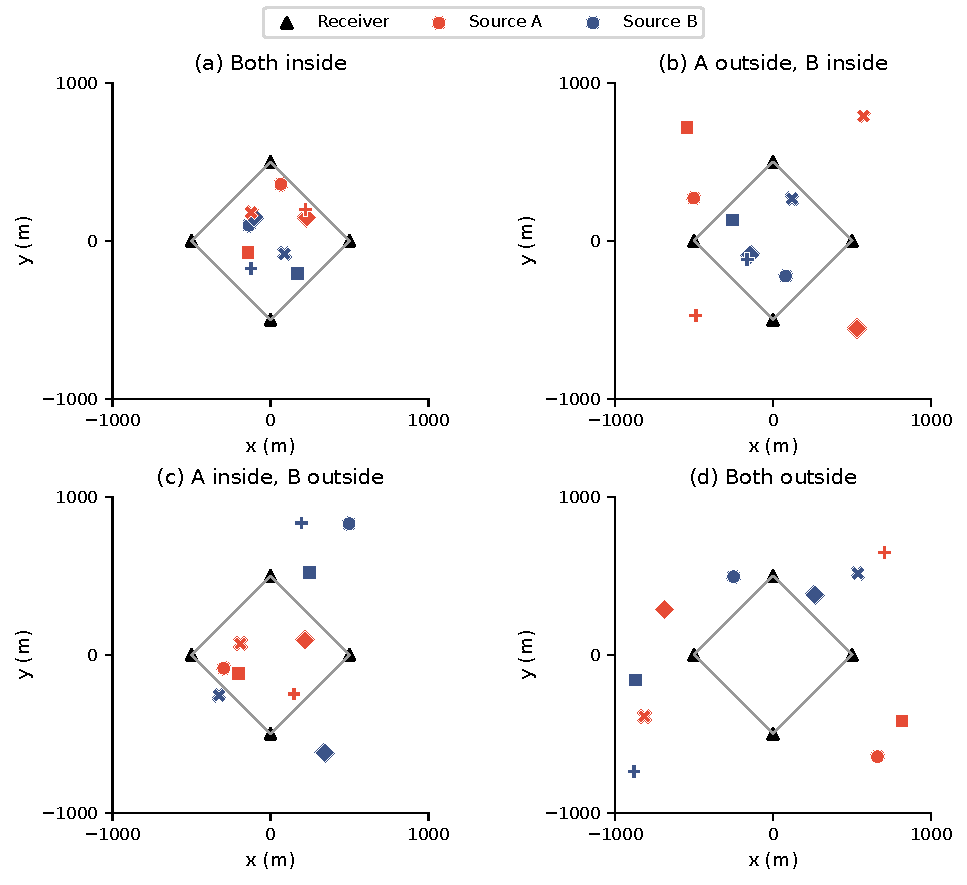
\includegraphics[width=.90\linewidth]{figures/formal_geometry.pdf}
\caption{Twenty source configurations, five per category. Black triangles denote stations. Matching shapes pair source A (red) and B (blue) within each panel; the diamond is the station convex hull.}\label{en:geometry}
\end{figure}

All methods share IQ data, propagation information, double-precision calculations and the initial grid. Their adapted objectives are specified below; native initialization and continuous refinement are retained.

AP branch refinements share projected-gradient tolerance $10^{-8}$ on the normalized objective, no objective-difference stopping term, and a 100-iteration local limit. VP-BNOMP and its fixed-coefficient reference use cyclic energy tolerance $10^{-8}$, at most five Newton steps per local call, a 50 m step cap, a 0.01 m local small-step exit and a 10,000-cycle safety limit. The different gradient and energy conditions are not equivalent optimization accuracies. Complete-method comparisons use their frozen native rules; joint-refinement and curvature comparisons match the relevant stopping conditions explicitly.

For $n$ observations indexed by $i$, one squared-distance assignment per observation \cite{Kuhn1955} determines errors for all reported position metrics:
\begin{equation}
\pi^*=\arg\min_\pi\sum_k\|\widehat{\bm p}_{\pi(k)}-\bm p_k\|^2,
\quad e_{ik}=\|\widehat{\bm p}_{i,\pi^*(k)}-\bm p_{ik}\|.
\end{equation}
RMSE is $\sqrt{n^{-1}\sum_i e_{ik}^2}$ and the empirical CDF is $n^{-1}\sum_i\mathbf1(e_{ik}\le t)$. Both include all observations. Two-source success requires $\max_k e_{ik}\le20$ m, a prescribed tolerance of $0.02R$ distinct from grid spacing. Invalid outputs remain failures in the denominator; all reported batches returned two finite positions.

Complete runtime includes the DFT, band selection, transfer, search, coefficient estimation, refinement and necessary output checks, with GPU synchronization. Adapter trajectory recording and final diagnostics are included where present; input-file reading, disk writes and offline statistics are excluded. Warm-up is separate. Runtime comparisons use the same batch for speedup ratios. The environment is Windows, Python 3.10.20, NumPy 2.2.6, PyTorch 2.8.0+cu129, an RTX 4070 Ti SUPER and 20 CPU threads, with double-precision responses and objectives. Resampling retains the six gaps of one realization as a group. Candidate-cost and curvature intervals condition on fixed layouts; broader hierarchical intervals are identified separately below.

\FloatBarrier
\subsection{Baseline objectives and implementation}
LS peaks continuously refines two separated maxima of \eqref{en:single}, without jointly fitting two sources. For covariance methods, split the same record into $S$ nonoverlapping segments of $N_s=N/S$ samples. With segment DFT $\bm z_{bf}\in\C^L$, normalized by $1/N_s$,
\begin{equation}
\widehat{\bm C}_f=S^{-1}\sum_{b=1}^S\bm z_{bf}\bm z_{bf}^H.
\end{equation}
The zero-mean model makes correlation and covariance equal. Segment noise variance is $\sigma_t^2/N_s$; only the same physical processing band is retained. No snapshots are pooled across realizations.

MUSIC requires $K<L$, independent response columns, full-rank source covariance and spatially white noise \cite{WeissAmar2005}. Let $\bm E_{n,f}$ contain the $L-K$ smallest-eigenvalue eigenvectors. The wideband score and noise-subtracted weights are
\begin{align}
S_{\rm MU}(\bm p)&=\left[\sum_f w_f\bm q_f^H
\bm E_{n,f}\bm E_{n,f}^H\bm q_f\right]^{-1},\\
\widetilde w_f&=\max\{\tr(\widehat{\bm C}_f)-L\sigma_t^2/N_s,0\},
\qquad w_f=\widetilde w_f/\sum_v\widetilde w_v.
\end{align}
Weights are uniform if their sum vanishes. Known $K$ fixes the subspace dimension, but finite-sample accuracy depends on effective snapshots and signal power at each bin.

MVDR minimizes $\bm h_f^H\bm C_{f,\delta}\bm h_f$ subject to $\bm h_f^H\bm q_f=1$, where $\bm h_f\in\C^L$ is a combining vector \cite{Capon1969}. Loading and wideband averaging give
\begin{equation}
\begin{split}
\bm C_{f,\delta}&=\widehat{\bm C}_f+
\delta\,\tr(\widehat{\bm C}_f)\bm I_L/L,\\
S_{\rm MV}(\bm p)&=F_s^{-1}\sum_f
[\bm q_f^H\bm C_{f,\delta}^{-1}\bm q_f]^{-1}.
\end{split}
\end{equation}
The dimensionless loading $\delta$ scales mean diagonal power. MVDR-known uses known relative responses and this frequency average, distinguished from the original DPD-HR formula \cite{TirerWeiss2016}.

For SBL, define the dictionary $\bm D_f=[\bm q_f(\bm g_1),\ldots,\bm q_f(\bm g_G)]$ and frequency coefficients $\bm z_f\sim\mathcal{CN}(0,\bm\Gamma)$, independent across frequencies with shared nonnegative powers $\bm\Gamma=\operatorname{diag}(\bm\gamma)$ \cite{Nannuru2019}. The covariance, posterior mean, negative log evidence and fixed-point update are
\begin{align}
\bm C_f&=\sigma_f^2\bm I_L+\bm D_f\bm\Gamma\bm D_f^H,\qquad
\bm\mu_f=\bm\Gamma\bm D_f^H\bm C_f^{-1}\bm x_f,\\
\mathcal E(\bm\gamma)&=F^{-1}\sum_f
[\log\det\bm C_f+\bm x_f^H\bm C_f^{-1}\bm x_f],\\
\gamma_j^+&=\gamma_j\left[
\frac{\sum_f|\bm d_{fj}^H\bm C_f^{-1}\bm x_f|^2}
{\sum_f\bm d_{fj}^H\bm C_f^{-1}\bm d_{fj}}
\right]^{1/2},
\end{align}
where $\bm d_{fj}$ is column $j$ of $\bm D_f$. Evidence backtracking controls updates. Every five iterations, eight active positions are optimized off-grid, allowing 20 m displacement per coordinate; L-BFGS-B uses coordinate scale 1,000 m and at most 20 iterations. Final peaks use individual $\gamma_j$. Every five iterations, stopping requires normalized evidence change below $10^{-5}$, relative $\ell_1$ power change below 1\%, and output/active-position motion below 0.05 m on two consecutive checks; the cap is 300 iterations.

Full AP repeatedly searches the conditional objective and refines positions, using five candidates and up to six outer cycles. Multistart ML minimizes $J$ from four unique spectral peak combinations and four Sobol spatial starts, removing unordered duplicates. GA-ML encodes four coordinates, with 128 individuals, four elites, size-three tournament selection, simulated binary crossover (probability 0.9, index 15), and polynomial mutation (per-coordinate probability 0.25, index 20) \cite{DebAgrawal1995}. It stops after 30 stagnant generations or 200 generations, then jointly refines the best individual.

The fixed-coefficient BNOMP direction differentiates
\begin{equation}
L_{\rm FC}(\bm p)=E_x^{-1}\sum_f
\|\bm y_f-\bm a_f(\bm p)q_f^{(0)}\|^2,
\label{en:fixedcoef}
\end{equation}
where $q_f^{(0)}$ is fitted at the current position, held fixed for differentiation and reference backtracking, and re-estimated after acceptance. The multi-frequency block structure follows \cite{Yang2022}; Hessian repair, bounds and backtracking are numerical safeguards. VP uses reduced curvature and reduced acceptance. Since original NOMP combines fixed-gain curvature with re-estimated-gain acceptance \cite{Mamandipoor2016}, we also isolate curvature by testing both directions with reduced acceptance.

MUSIC uses four segments; MVDR-known uses eight and $\delta=0.01$. AP local calls allow 25 line-search trials and 100 iterations; alternating refinement allows 12 sweeps and initial single-source refinement uses relative tolerance $10^{-12}$. BNOMP floors Hessian eigenvalues at $10^{-9}$ and tries step factors $1,1/2,1/4,1/8,1/16$ within the search bounds. Its other limits and AP's common gradient tolerance were specified above. Parameters are fixed before the reported comparisons.

\FloatBarrier
\subsection{Common-data comparison and expanded evaluation}
Table~\ref{en:common} compares all methods on the same 240 observations. MCJ-AP matches the complete recovery of full AP and SBL at substantially lower complete cost. SBL has a wider weak-source error distribution. The two BNOMP versions recover the same 228 observations, with lower mean cost for the waveform-eliminated version.
\begin{table}[pos=H]\centering\small
\caption{Common 240 observations. RMSE in m; runtime mean, median and P95 in s. Every metric includes all observations.}\label{en:common}
\begin{tabular}{@{}lrrrrrr@{}}\toprule
Method & Success/240 & RMSE A & RMSE B & Mean & Median & P95\\\midrule
LS peaks & 38 & 191.982 & 845.184 & 0.2368 & 0.2181 & 0.3297\\
WB-MUSIC & 151 & 93.515 & 646.892 & 0.2015 & 0.1893 & 0.2719\\
MVDR-known & 75 & 320.684 & 804.082 & 0.1925 & 0.1807 & 0.2625\\
Full AP & 240 & 0.876 & 1.596 & 8.9076 & 9.1483 & 12.2348\\
Fixed BNOMP & 228 & 0.906 & 89.706 & 2.9416 & 1.4625 & 8.1989\\
VP-BNOMP & 228 & 0.875 & 86.177 & 0.5907 & 0.3921 & 1.3971\\
Multistart ML & 45 & 256.061 & 776.935 & 1.2227 & 1.0868 & 2.5595\\
GA-ML & 185 & 279.056 & 501.231 & 8.0702 & 8.1102 & 9.0229\\
WB-SBL & 240 & 1.096 & 3.743 & 44.1296 & 36.8237 & 97.7075\\
MCJ-AP ($M=5$) & 240 & 0.876 & 1.596 & 0.7081 & 0.6347 & 1.0232\\\bottomrule
\end{tabular}\end{table}

\begin{figure}[pos=H]\centering
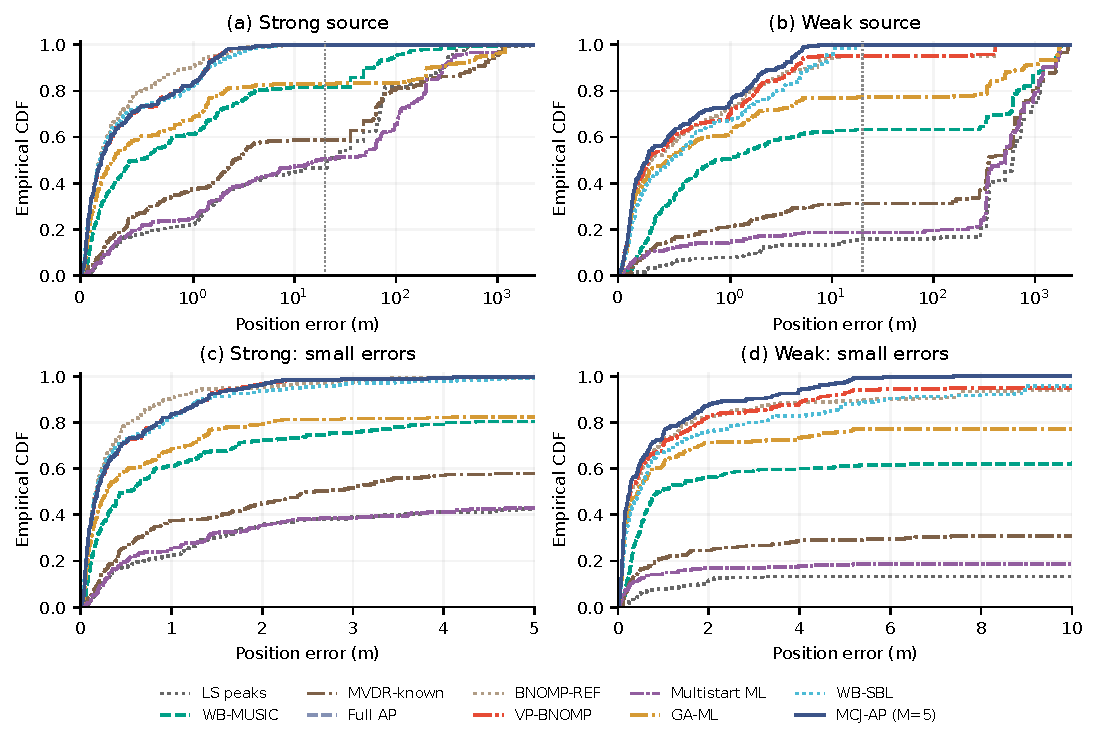
\includegraphics[width=\linewidth]{figures/assignment_cost_20261019/common_error_cdf.pdf}
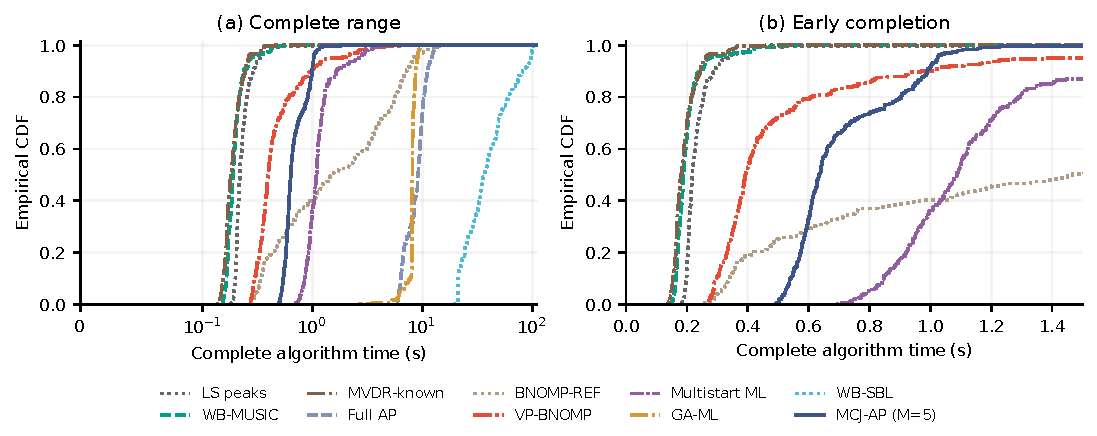
\includegraphics[width=\linewidth]{figures/assignment_cost_20261019/common_time_cdf.pdf}
\caption{Error and complete-runtime CDFs on the common 240 observations. The error panels show full ranges and small-error enlargements; the time panels show the full range and early completion. Full-range axes are linear near zero and logarithmic beyond their thresholds. Vertical error lines indicate 20 m. All curves retain the full denominator.}\label{en:commoncdf}
\end{figure}
Figure~\ref{en:commoncdf} distinguishes typical precision from large-error tails. The AP error curves nearly coincide. VP-BNOMP is accurate on most observations, but retains a distant weak-source tail and occasional long runtimes. Spectral methods are fast, yet their failures involve large errors rather than small threshold crossings.

\begin{figure}[pos=H]\centering
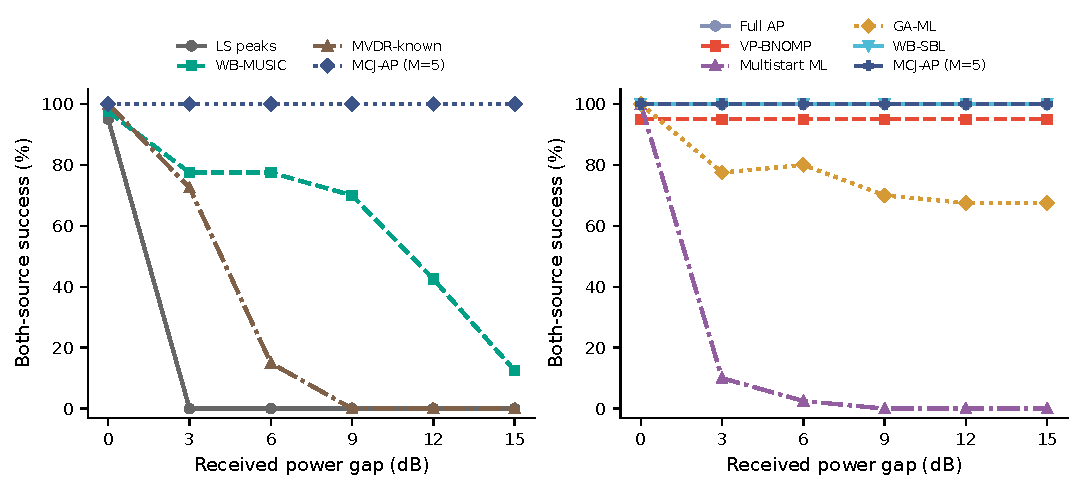
\includegraphics[width=\linewidth]{figures/formal_common.pdf}
\caption{Power-gap sweep on the common subset, 40 observations per gap. Both panels use the same five-candidate AP reference.}\label{en:power}
\end{figure}
As the power gap increases, MUSIC and MVDR-known lose recovery (Fig.~\ref{en:power}); Section~\ref{en:windowcheck} examines whether finite-window mismatch explains the tested failures. Full AP and multistart ML optimize the same joint objective but have very different outcomes, demonstrating the importance of initialization and search. GA reaches its generation limit in 208 observations and SBL in 14; the other methods have no limit exits. All outputs remain included.

\begin{figure}[pos=H]\centering
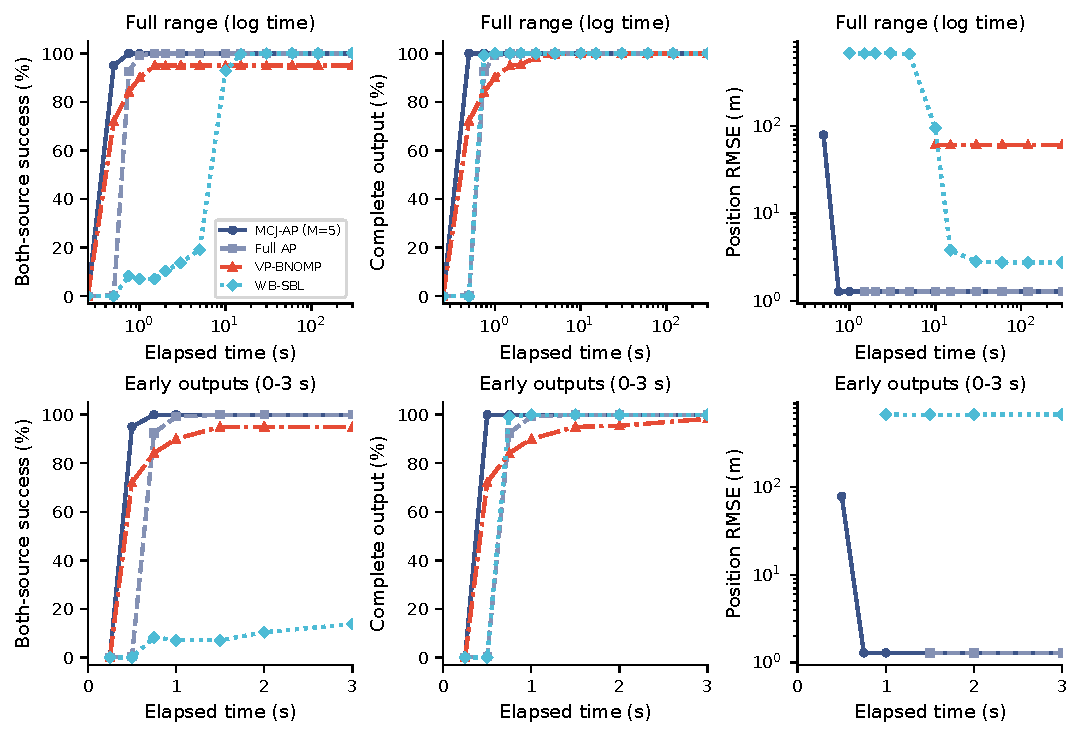
\includegraphics[width=\linewidth]{figures/formal_time.pdf}
\caption{Saved output trajectories on 240 observations. Upper panels use logarithmic time; lower panels enlarge 0--3 s. Columns show two-source success, complete-output fraction and pooled RMSE. Missing outputs count as unsuccessful; RMSE is shown after all observations have outputs.}\label{en:time}
\end{figure}
Five-candidate AP, full AP and SBL first reach complete success at saved times of 0.75, 1.5 and 30 s (Fig.~\ref{en:time}). Connected checkpoints do not define new stopping rules. VP publishes only its final complete output in this batch, so its curve does not expose intermediate cycles.

\begin{table}[pos=H]\centering\small
\caption{Expanded 2,400-observation evaluation. RMSE in m and complete time in s. VP-BNOMP timing is from a separate same-input batch; controlled speedups are evaluated in paired batches.}\label{en:core}
\begin{tabular}{@{}lrrrrrr@{}}\toprule
Method & Success/2400 & RMSE A & RMSE B & Mean & Median & P95\\\midrule
AP ($M=1$) & 2280 & 0.897 & 107.265 & 0.3958 & 0.3700 & 0.5104\\
AP ($M=2$) & 2280 & 0.897 & 103.698 & 0.4704 & 0.4329 & 0.6340\\
MCJ-AP ($M=5$) & 2376 & 0.896 & 46.984 & 0.7180 & 0.6495 & 1.0267\\
VP-BNOMP & 2278 & 0.892 & 74.193 & 0.5855 & 0.3693 & 1.2470\\\bottomrule
\end{tabular}\end{table}
On 2,400 observations, five candidates increase AP success from 95\% to 99\% (Table~\ref{en:core}). Hierarchical resampling gives a 95\% interval of [96.83\%,100\%] for its success rate. The four-percentage-point increase over two candidates has interval [0,12.17] percentage points, reflecting concentration in one configuration. The common 240 subset and expanded cohort are reported separately rather than counted as independent observations.

\begin{figure}[pos=H]\centering
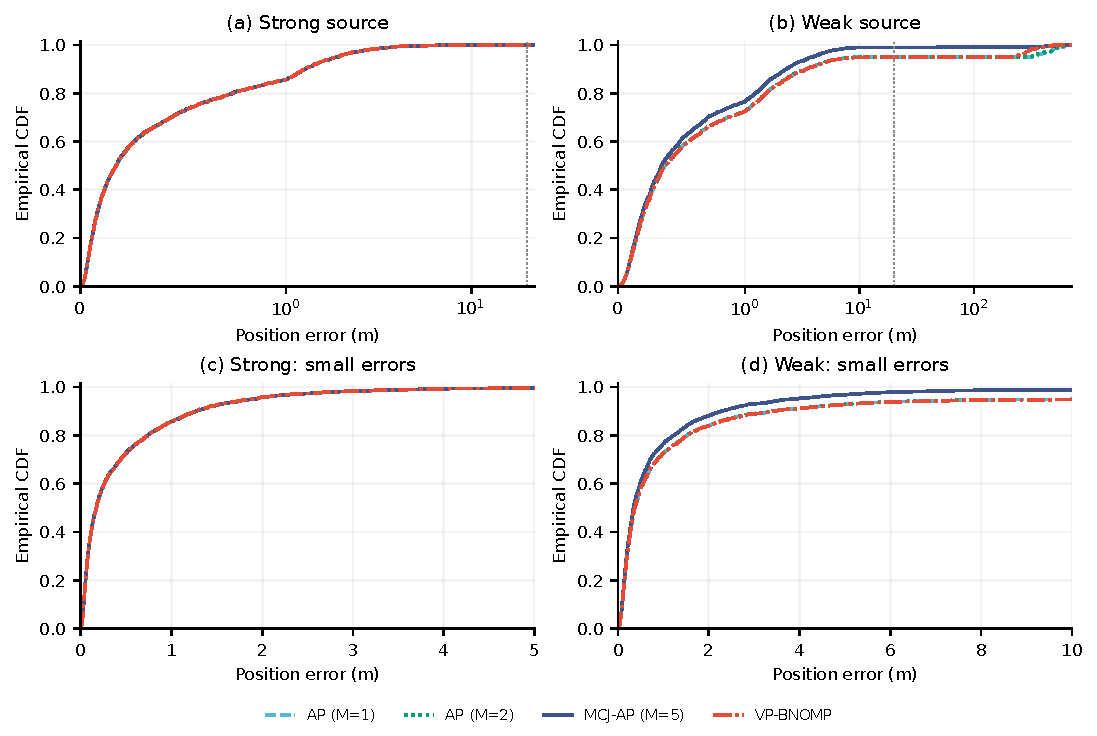
\includegraphics[width=\linewidth]{figures/assignment_cost_20261019/core_error_cdf.pdf}
\caption{Strong- and weak-source error CDFs for all 2,400 core observations. Upper panels cover full ranges and lower panels enlarge small errors. All observations, including failures, remain in each curve.}\label{en:corecdf}
\end{figure}
The strong-source CDFs nearly coincide (Fig.~\ref{en:corecdf}). Small weak-source errors are also similar, whereas tails differ. Five-candidate AP has weak-source P95 of 3.85 m but RMSE of 46.98 m. Configuration 4 accounts for all 24 failures and over 99.7\% of its weak-source squared error in each power bin.
\begin{figure}[pos=H]\centering
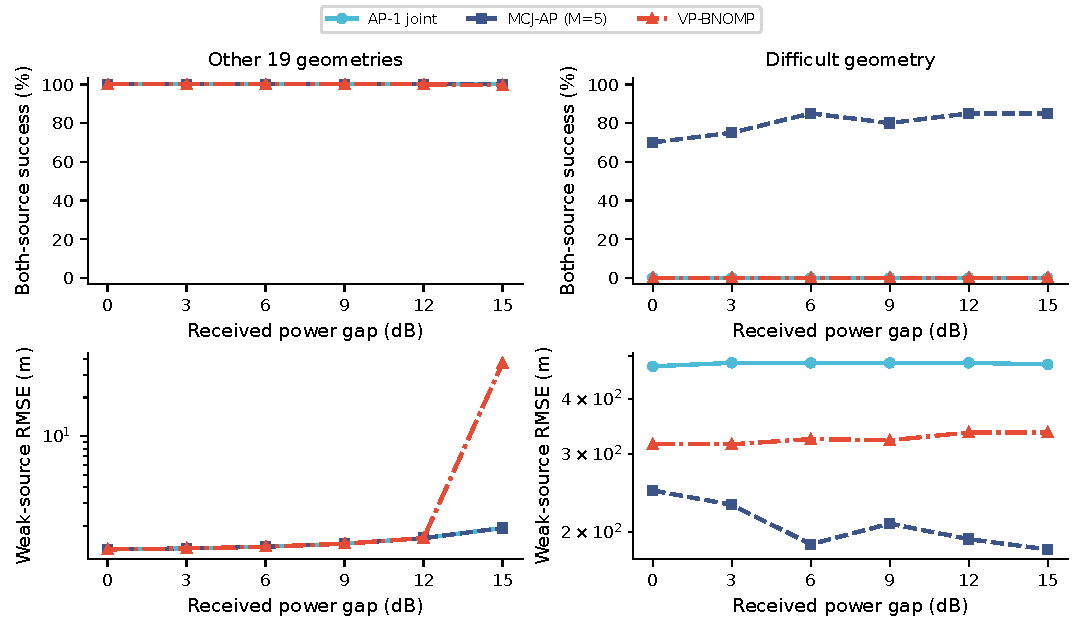
\includegraphics[width=.92\linewidth]{figures/formal_core.pdf}
\caption{Power-gap results for the other 19 configurations (2,280 observations) and configuration 4 (120 observations). This diagnostic grouping leaves all observations in the overall results.}\label{en:powergroups}
\end{figure}
In the other configurations, AP weak-source RMSE rises from 1.31 to 1.93 m across the power sweep (Fig.~\ref{en:powergroups}). VP has two failures in configuration 1 at 15 dB, producing 15.25 m RMSE over those 19 configurations versus about 1.52 m for AP. In configuration 4, VP reduces weak-source RMSE from single-candidate AP's 479.66 m to 325.07 m without meeting the 20 m tolerance. Configuration 4 drives the nonmonotone overall RMSE; geometry is unchanged across power bins.

\FloatBarrier
\subsection{Candidate coverage and joint-refinement cost}
The 96 AP recoveries occur in configuration 4 and involve 18 of its 20 waveform/noise realizations. Single-candidate AP fails on all 120 observations there, whereas five candidates recover 96. No observation is changed from success to failure in the other configurations. Saved branch results show that exactly 2,376 observations have at least one successful refined branch, and final residual selection chooses a successful branch in every such observation. The remaining 24 have no successful branch among the five refined candidates.

\begin{figure}[pos=H]\centering
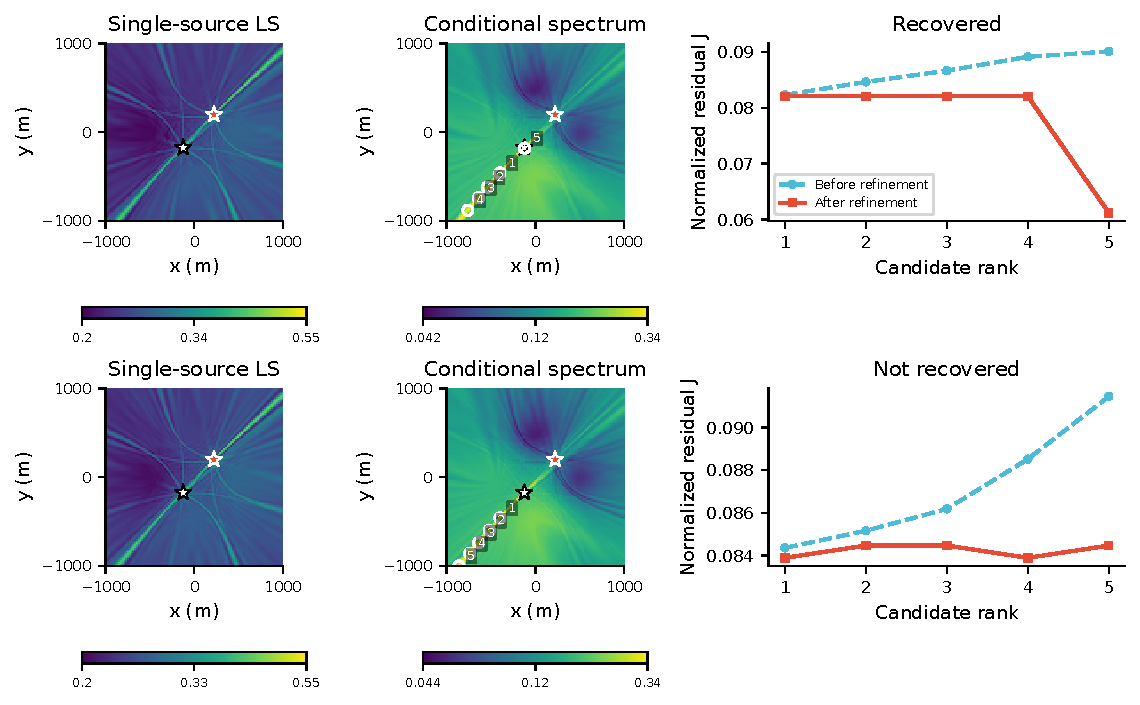
\includegraphics[width=\linewidth]{figures/formal_candidates.pdf}
\caption{Two post hoc cases from configuration 4 at 0 dB. Columns show the single-source spectrum, conditional spectrum and pre-/post-refinement branch residuals. The upper case is recovered by the fifth candidate; the lower case has no effective candidate. Lines in the right panels connect branch indices, not optimization trajectories.}\label{en:cases}
\end{figure}
In the upper case of Fig.~\ref{en:cases}, the first four branches enter a distant region; the fifth gives a lower final residual and approximately 0.09 m weak-source error. In the lower case, even the nearest candidate is about 397 m from source B and refinement cannot recover it. These cases explain why retaining candidates can help while local refinement alone cannot repair missing coverage.

\begin{figure}[pos=H]\centering
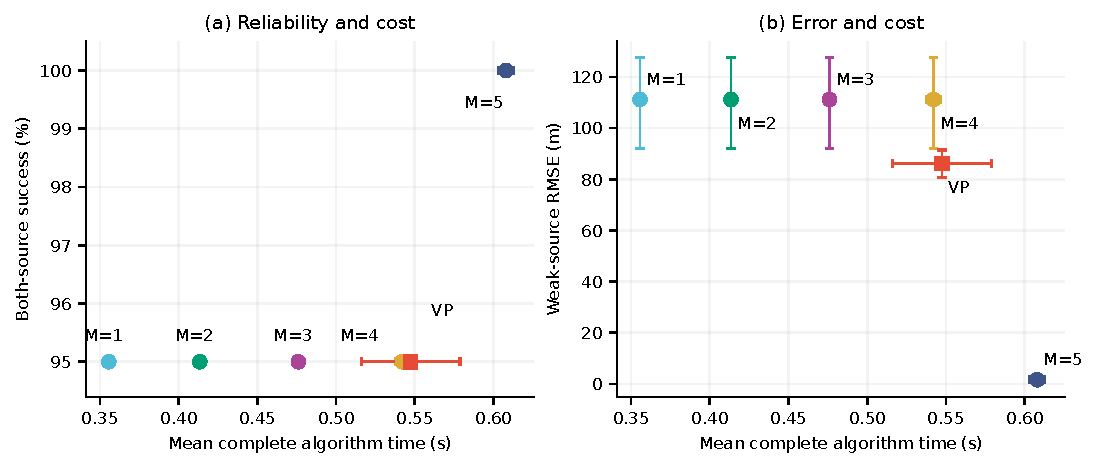
\includegraphics[width=\linewidth]{figures/assignment_cost_20261019/candidate_tradeoff.pdf}
\caption{Candidate count versus complete mean runtime, success and weak-source RMSE on 240 observations, measured in one interleaved batch. Error bars are 95\% paired intervals resampling realizations within fixed layouts while retaining the six gaps together.}\label{en:tradeoff}
\end{figure}
In this batch, $M=1$--4 each succeeds on 228 observations; mean runtime increases from 0.3556 to 0.5420 s and weak-source RMSE remains about 111.2 m. VP-BNOMP has 228 successes, 86.18 m weak-source RMSE and 0.5474 s mean runtime. Five-candidate AP succeeds throughout at 0.6079 s and 1.60 m weak-source RMSE. VP median time is 0.3674 s versus single-candidate AP's 0.3514 s; its P95 is 1.3147 s versus five-candidate AP's 0.7201 s. Among 228 common successes, VP is faster than five-candidate AP in 197; five candidates recover the other 12 observations. These results distinguish typical speed from recovery and runtime tails. Saved full-cohort prefixes give 2,281 and 2,289 successes for three and four candidates, respectively; these are position-only replays.

\begin{table}[pos=H]\centering\small
\caption{Paired alternating and joint refinement of the same five candidates on 2,400 observations. Both selected outputs meet the same projected-gradient tolerance.}\label{en:apjoint}
\begin{tabular}{@{}lrrrrr@{}}\toprule
Refinement & Success & RMSE B/m & Mean time/s & $J$ calls & Gradient calls\\\midrule
Alternating & 2376 & 46.983 & 1.0840 & 204.21 & 198.21\\
Joint & 2376 & 46.984 & 0.7441 & 120.36 & 114.36\\\bottomrule
\end{tabular}\end{table}
Table~\ref{en:apjoint} isolates the cost of refinement from candidate coverage. Success/failure identities agree observation by observation, strong-source RMSE is about 0.896 m, and weak-source P95 is about 3.85 m for both. Joint refinement reduces mean complete time by 31.36\% and gradient calls by 42.30\%. The paired hierarchical 95\% interval for joint-minus-alternating time is $[-0.3691,-0.3121]$ s. Every configuration has lower mean cost, with savings from 11.42\% to 48.04\%. Two unselected alternating branches reach the local safety limit and remain included. Candidate retention supplies additional starts; joint refinement processes them with fewer calls at matched accuracy.

\FloatBarrier
\subsection{Isolating waveform-eliminated curvature}
The common-data fixed-coefficient/VP comparison in Table~\ref{en:common} changes both local curvature and the trial acceptance objective, reducing mean runtime by 79.92\%. To isolate curvature, a separate paired batch applies the same waveform-eliminated objective $\phi_j$ to trial acceptance. FC--VP computes directions with $H_{zz}$ and VP--VP with $H_{\rm VP}$. Both use the same current conditional coefficient estimate, gradient, discovery sequence, safeguards, backtracking and cyclic energy stopping rule.
\begin{table}[pos=H]\centering\small
\caption{Curvature comparison with a common waveform-eliminated acceptance objective, 240 paired observations. Update and cycle counts are means per observation.}\label{en:curvaturetable}
\begin{tabular}{@{}lrrrrrr@{}}\toprule
Version & Success & RMSE A/m & RMSE B/m & Mean time/s & Updates & Cycles\\\midrule
FC--VP & 228/240 & 0.906 & 89.706 & 5.574 & 1498.82 & 810.90\\
VP--VP & 228/240 & 0.875 & 86.177 & 0.905 & 135.55 & 47.97\\\bottomrule
\end{tabular}\end{table}
Success/failure identities agree and all outputs stop under the native energy rule. Mean complete runtime falls by 83.77\%, with fixed-layout paired 95\% interval [81.73\%,85.58\%]. Median time falls from 2.836 to 0.567 s and P95 from 16.161 to 2.538 s. VP--VP is faster in 170 of 240 observations: the mean saving is driven especially by reductions in slow cases. The associated update and cycle reductions support the curvature mechanism in \eqref{en:rate}.

Mean core times are 5.5483 and 0.8987 s; recording and final checks add 0.0254 and 0.0059 s. Audits of 480 historical/current VP pairs find matching inputs, positions, objectives, counts, stopping reasons and saved paths despite different absolute wall times. Each speedup therefore uses its own paired batch: 79.92\% measures the complete local-update change, while 83.77\% isolates curvature under common acceptance. The latter interval uses 4,000 within-configuration paired bootstrap draws (seed 20261020), retaining all six gaps of a realization. Equal energy thresholds do not imply equal final joint-gradient accuracy; Section~\ref{en:localchecks} examines that distinction.

\FloatBarrier
\subsection{Frozen methods at new source positions}
Table~\ref{en:new} and Fig.~\ref{en:newcdf} assess the 16 new source configurations. Both AP variants recover all 480 observations with nearly identical errors, while five candidates cost approximately 1.96 times as much as one. The first branch is already effective, so additional branches do not increase success. Together with configuration 4, this identifies candidate retention as a cost-for-coverage choice whose recovery benefit depends on initialization.
\begin{table}[pos=H]\centering\small
\caption{New source configurations, 480 observations; receiver positions unchanged. RMSE in m and complete runtime in s.}\label{en:new}
\begin{tabular}{@{}lrrrrrr@{}}\toprule
Method & Success/480 & RMSE A & RMSE B & Mean & Median & P95\\\midrule
AP ($M=1$) & 480 & 0.958 & 2.194 & 0.461 & 0.456 & 0.545\\
MCJ-AP ($M=5$) & 480 & 0.958 & 2.194 & 0.906 & 0.893 & 1.078\\
VP-BNOMP & 390 & 202.882 & 206.261 & 1.051 & 0.629 & 4.245\\\bottomrule
\end{tabular}\end{table}
\begin{figure}[pos=H]\centering
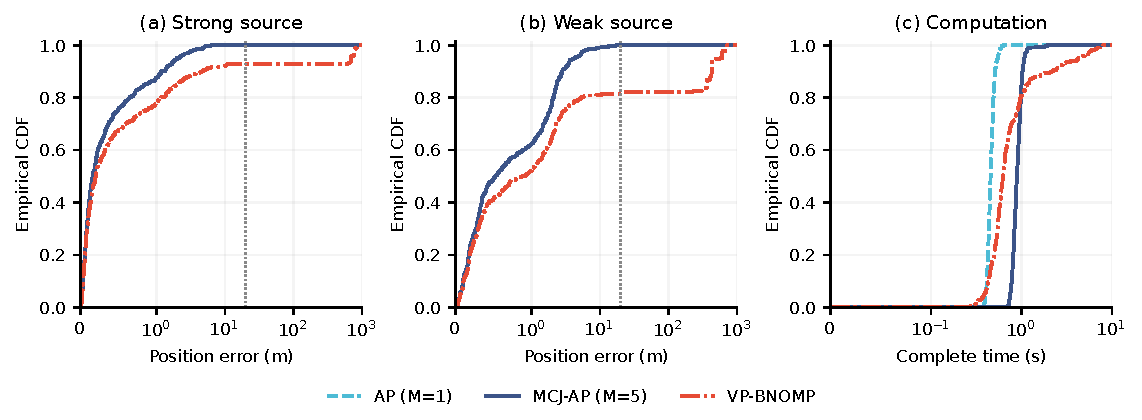
\includegraphics[width=\linewidth]{figures/review_supplement_20261020/independent_cdf.pdf}
\caption{Error and complete-runtime CDFs on the 480 new observations. AP error curves nearly overlap. All observations are retained; error reference lines mark 20 m. Full-range axes are linear near zero and logarithmic beyond the stated thresholds.}\label{en:newcdf}
\end{figure}
VP-BNOMP has 90 failures in new configurations 8, 9, 14 and 15: 30, 25, 30 and 5, respectively. Every gap has 15 failures; 55 involve only B, 33 both sources and two only A. All five realizations are represented. Failed observations average 1.448 s versus 0.959 s for successful ones; they stop by energy stability, with larger final objectives than AP. They already fail at the first saved full pair and never subsequently succeed. Thus neither a discarded saved success nor safety-limit truncation explains the failures. Because recording begins after one two-source cycle, it does not distinguish failed discovery from a particular update.

\FloatBarrier
\subsection{Finite-window and numerical checks}
\label{en:windowcheck}
Eight development observations (four configurations at 0 and 15 dB) provide saved clean source components. At the true positions, the finite-window residual and expected projected noise energy are
\begin{equation}
E_{\rm win}=\sum_{b,f}\|\bm\Pi_{\bm A_f}^{\perp}\bm z_{bf}^{(0)}\|^2,
\qquad E_n=SF_s(L-K)\sigma_t^2/N_s.
\end{equation}
Every $\bm A_f$ is full column rank. For one, four and eight segments, respectively, the residual fractions are 0.209--0.382\%, 0.756--1.387\% and 1.529--2.854\%; the corresponding $E_{\rm win}/E_n$ ranges are 0.035--0.882, 0.126--3.210 and 0.238--6.611. Shorter windows increase the mismatch.

Rectangular and periodic Hann windows were compared with a 4,096-sample Hann window using four overlapping frames. Windowed noise variance is $\sigma_t^2\sum_n w[n]^2/N_s^2$; overlapping frames are not independent snapshots. At 15 dB, the long window reduces $E_{\rm win}/E_n$ to 0.076--0.294, but MUSIC and MVDR-known still recover only 1/4 and 0/4 observations, retaining the original failures. Both recover 4/4 at 0 dB. Projecting each clean source onto its true response before restoring the original noise removes almost all model residual, yet none of the seven failed method--observation pairs recovers. This truth-assisted diagnostic is excluded from ranking. Finite-window mismatch alone does not explain the tested failures.

\label{en:localchecks}
Numerical convergence was also checked separately from localization error. Continuing native VP paths on eight development observations until the joint projected gradient reaches $10^{-8}$ keeps success at 8/8, changes weak-source RMSE from 3.22 to 3.25 m and raises mean complete time, including gradient checks, from 0.382 to 0.860 s.

The fixed-coefficient small-step mechanism was examined on eight observations. With cyclic energy tolerances $10^{-8}$, $10^{-7}$ and $10^{-6}$, successes are 8/8, 7/8 and 6/8; mean times are 5.478, 2.318 and 0.971 s, and derivative calls are 2679.5, 1133.9 and 467.4. Removing only the small-step local exit gives 8/8 at 8.011 s and 4758.4 calls; waveform elimination at $10^{-8}$ gives 8/8 at 0.436 s and 70.4 calls. All 21,436 reference updates are accepted, 83.67\% shorter than 0.01 m, without Hessian repair, step clipping, backtracking reduction or boundary clipping. At two outside-source diagnostic positions, raw steps increase from 0.0138/0.0111 m to 11.25/32.26 m after elimination, before backtracking. At four saved positions, analytic reduced Hessians match automatic differentiation within about $1.4\times10^{-18}$ maximum absolute difference. These checks motivate the formal curvature pair; they are not substitutes for its complete cost measurements.

\FloatBarrier
\section{Conclusions}
For unknown overlapping wideband sources, candidate coverage and position--waveform coupling affect different parts of direct localization. MCJ-AP retains conditional candidates, jointly refines each pair and selects the final residual. It raises two-source success from 95\% to 99\% on 2,400 observations, while matched-accuracy joint refinement reduces the cost of processing five candidates by 31.36\%. VP-BNOMP removes waveform coupling from local curvature; a common-acceptance paired comparison reduces mean runtime by 83.77\%, together with fewer local updates and cycles. On new source configurations, AP remains reliable but extra candidates provide no additional recovery, and VP retains configuration-dependent failures. Candidate retention therefore supplies conditional recovery benefits, whereas reduced curvature supplies a local efficiency benefit. The conclusions concern known two-source count, synchronized stations and the matched baseband propagation model. Candidate allocation and unknown source count provide directions for further work.

% Before submission, the authors must confirm authorship, affiliations, funding,
% competing interests, data/code availability and the applicable AI-use statement.
% No such declarations are inferred from the research results.
\FloatBarrier
\appendix
\FloatBarrier
\section{New source coordinates}\label{en:coordinates}
Table~\ref{en:coordinates-table} lists the new positions in meters to six decimal places. Categories 1--4 correspond to both inside, A outside/B inside, A inside/B outside, and both outside the receiver convex hull. Geometry and waveform seeds are 20261020071 and 20261020072; realization identifiers are 1000--1004. Configuration numbers are one-based. These positions obey the same geometric exclusions as the original cohort and were not screened by method performance.
\begin{table}[pos=H]\centering
\caption{New source positions. A is power-scaled; B and the noise are fixed.}\label{en:coordinates-table}
\begin{tabular}{@{}rrrrrr@{}}\toprule
No. & Category & $x_A$ & $y_A$ & $x_B$ & $y_B$\\\midrule
1 & 1 & -209.742960 & -211.672998 & -135.426339 & 121.578497\\
2 & 1 & -115.361316 & 76.809910 & 67.769590 & -192.728293\\
3 & 1 & -208.559801 & 115.499630 & 268.616751 & -92.726639\\
4 & 1 & 173.459164 & -110.441904 & -168.154517 & -145.923194\\
5 & 2 & -926.529606 & 771.380729 & -198.481435 & 152.456653\\
6 & 2 & -628.314566 & -929.843027 & -55.519139 & -297.939120\\
7 & 2 & -195.757938 & -496.419920 & 157.528284 & 224.885259\\
8 & 2 & -734.894082 & -306.033731 & -249.535479 & 71.485648\\
9 & 3 & -64.564529 & 351.783227 & 663.100329 & 428.023655\\
10 & 3 & -166.451414 & 260.105867 & 823.995321 & 431.176047\\
11 & 3 & 74.808116 & 299.580428 & -702.622192 & 474.464614\\
12 & 3 & -162.472651 & -112.907043 & 765.537745 & -808.531366\\
13 & 4 & 313.792247 & 602.900501 & 700.222844 & -274.728424\\
14 & 4 & 482.010461 & 239.752856 & 888.180085 & 90.857032\\
15 & 4 & -374.838719 & 599.269525 & 240.800462 & 663.866438\\
16 & 4 & 624.598019 & 542.011213 & -163.287363 & 904.989973\\\bottomrule
\end{tabular}\end{table}
\FloatBarrier
\bibliographystyle{\PaperRoot template/cas-model2-names}
\bibliography{\PaperRoot references/references}
\end{document}
